%include exam documentclass
\documentclass{exam} 
\usepackage{fullpage}
\usepackage{amsmath}
\usepackage{comment}
\usepackage{graphicx}

\begin{document}

%print header
\examheader{CISC 106}{UEF Example}{Developed: 2010}

%example of a block
\begin{block}{example topic}
  This is an example of a block
\end{block}

%example figure
\begin{figure}[placement h]
  \begin{center}
      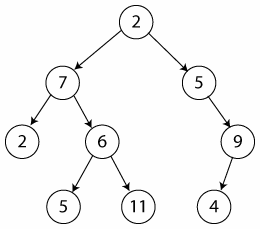
\includegraphics[scale=0.50]{binary_tree.png}
      \caption{Example Figure}
      \label{fig:example topic}
   \end{center}
\end{figure}

%example of a problem, require block:example topic
%and fig:example topic
\begin{problem}[require=example topic]{example topic}{15}
  This is a problem
  \ref{fig:example topic}
  \begin{answers}
    \answer[correct] correct answer 1
    \answer answer 2
    \answer[fixed] fixed answer 3
    \answer[correct,fixed] correct fixed answer 4
    \answer answer 5
    \answer[fixed,correct] fixed correct answer 6
  \end{answers}
\end{problem}

\begin{block}{logical}
The following problems relate to logical situations.
\end{block}

\begin{problem}[requires=logical]{logical}{10} 
  Which expression tests whether
  variable x is between (but not the same as) the values 5 and 10.
%:type  logical
  \begin{answers}
    \answer \verb+5 < x < 10+
    \answer \verb+5 <= x <= 10+
    \answer \verb+5 < x & x > 10 +
    \answer[correct] \verb+x < 10 & 5 < x+ %correct answer
    \answer[fixed] none of these  %fixed position
  \end{answers}
\end{problem}

\begin{problem}[requires=logical]{logical}{5} 
  Which of the following is a MATLAB expression for testing ``x is
  outside the range from 3 to 5'' (the range includes 3 and 5)? 
%:type logical
  \begin{answers}  
    \answer \verb@3 > x & x > 5@
    \answer \verb@3 > x | x < 5@
    \answer[correct] \verb@3 > x | x > 5@ %correct answer
    \answer[fixed] cannot be expressed in MATLAB %fixed position
    \answer[fixed] none of the above %fixed position
  \end{answers}
\end{problem}

\begin{problem}[requires=logical]{logical}{5} 
  Which of the following is a MATLAB expression for testing ``x is
  outside the range from 3 to 5'' (the range includes 3 and 5)? 
%:type logical
  \begin{answers}  
    \answer \verb@3 > x & x > 5@
    \answer \verb@3 > x | x < 5@
    \answer[correct] \verb@3 > x | x > 5@ %correct answer
    \answer[fixed] cannot be expressed in MATLAB %fixed position
    \answer[fixed] none of the above %fixed position
  \end{answers}
\end{problem}

\begin{problem}[requires=matrix matlab]{matrix matlab}{7}
  Suppose you have a matrix x = \footnotesize
  $\begin{array}{ccc}1 & 2 & 3 \\4 & 5 & 6 \end{array}$
  \normalsize. Which of the following will evaluate to 6?
%:type  matrix matlab
`  \begin{answers}   
    \answer x(3,2)
    \answer x(1,2)
    \answer x[2,2]
    \answer x[2,3] 
    \answer[correct,fixed] none of these %correct answer, fixed position
  \end{answers}
\end{problem}

\begin{problem}[require=logical]{logical}{8} 
  In MATLAB the value 1 is true, and true is:
%:type logical
  \begin{answers} 
    \answer there are no boolean types in MATLAB
    \answer[correct] any value that isn't zero %correct answer
    \answer 1
    \answer 0
    \answer[fixed] none of the above %fixed position
  \end{answers}
\end{problem}

\begin{block}{fooblock}
This block was inputted by Jesse and Kyle for testing.
\end{block}

\begin{problem}[require=fooblock]{fooblock}{8} 
This is a problem, the correct answer is not a, b, or c.
%:type logical
  \begin{answers} 
    \answer a
    \answer b
    \answer c
    \answer [correct] d %correct
    \answer[fixed] none of the above %fixed position
  \end{answers}
\end{problem}

\begin{problem}[require=fooblock]{fooblock}{8} 
What is the answer to 6 * 7?
%:type logical
  \begin{answers} 
    \answer 84 / 2 + 16
    \answer 67 mod 9
    \answer [correct] 21 * 2 %correct
    \answer The answer is, like, the answer, man.
    \answer[fixed] none of the above %fixed position
  \end{answers}
\end{problem}


\begin{problem}[require=noblock]{noblock}{8} 
What is the answer to 6 * 7?
%:type logical
  \begin{answers} 
    \answer 84 / 2 + 16
    \answer 67 mod 9
    \answer [correct] 21 * 2 %correct
    \answer The answer is, like, the answer, man.
    \answer[fixed] none of the above %fixed position
  \end{answers}
\end{problem}

\begin{block}{matrix matlab}
The following problems relate to matrix operations done in matlab.
\end{block}

\begin{problem}[requires=matrix matlab]{matrix matlab}{3}
 Suppose you have a matrix x = \footnotesize
$\begin{array}{cccc}1 & 2 & 3 & 4\\3 & 4 & 5 & 6\end{array}$
\normalsize. Which of the following will evaluate to \footnotesize
$\begin{array}{c}3 \\ 5\end{array}$\normalsize?
%:type  matrix matlab
  \begin{answers}   
    \answer x(3)
    \answer x(3,:)
    \answer x[:,3]
    \answer[correct] x(:,3) %correct answer
    \answer[fixed] none of these %fixed position
   \end{answers}
\end{problem}

\begin{problem}[requires=matrix matlab]{matrix matlab}{4} 
  Which of the following will extract \texttt{[5 6 7]} from the matrix m
  shown?\\
\texttt{>> m = [3 4 5 6 7 8];
}
%\myans{A}{B}{E}
  \begin{answers}
    \answer[correct] m(3:5) %correct answer
    \answer m(5:end-1)
    \answer m(end-1:5)
    \answer m[5, 7]
    \answer[fixed] none of these %fixed position
  \end{answers}
\end{problem}


\begin{problem}[requires=matrix matlab]{matrix matlab}{8}
  Suppose you have a matrix x = \footnotesize
  $\begin{array}{cccccc}1 & 2 & 3 & 4 & 5 & 6 \end{array}$
  \normalsize. Which of the following will evaluate to \footnotesize
  $\begin{array}{cccccc}1 & 2 & 3 & 4 & 5 \end{array}$\normalsize?
%:type  matrix matlab
  \begin{answers}   
    \answer x(1,end)  
    \answer x(end-1)  
    \answer[correct] x(1,end-1) %correct answer
    \answer x(1,1-end)
    \answer[fixed] none of these %fixed position
  \end{answers}
\end{problem}

\begin{problem}[requires=matrix matlab]{matrix matlab}{7}
  Suppose you have a matrix x = \footnotesize
  $\begin{array}{ccc}1 & 2 & 3 \\4 & 5 & 6 \end{array}$
  \normalsize. Which of the following will evaluate to 6?
%:type  matrix matlab
`  \begin{answers}   
    \answer x(3,2)
    \answer x(1,2)
    \answer x[2,2]
    \answer x[2,3] 
    \answer[correct,fixed] none of these %correct answer, fixed position
  \end{answers}
\end{problem}

\begin{problem}{function call}{15}
  Consider the function f:
  \begin{verbatim}
    function answer = f(a)
    answer = a+2;
    end
  \end{verbatim}
  What will be in x after the command:
  \begin{verbatim}>> x = f(4);
  \end{verbatim}
%:type function call
  \begin{answers}
    \answer[correct] 6 %correct answer
    \answer 4
    \answer f(4)
    \answer[fixed] error %fixed position 
    \answer[fixed] none of these %fixed position
  \end{answers}
\end{problem}

\begin{problem}{function call}{5}
  Consider the function f:
  \begin{verbatim}
    function [] = f(x)
    output = 7;
    end
  \end{verbatim}
  What will be in x after the command:
  \begin{verbatim}>> x = f(3);\end{verbatim}
%:type function call
  \begin{answers}
    \answer 7
    \answer f(7)
    \answer ans
    \answer[fixed,correct] error %correct answer, fixed position
    \answer[fixed] none of these %fixed position
  \end{answers}
\end{problem}

%goodbye message block
\begin{block}{Goodbye Message}
  Did you remember to write your name on the first page?  Did you
  attempt to answer every question?    Have a good holiday.
\end{block}

\end{document}







